\documentclass[border=.2cm]{standalone}
\usepackage{tikz}
\usepackage{amsmath}
\usetikzlibrary{angles}

\begin{document}

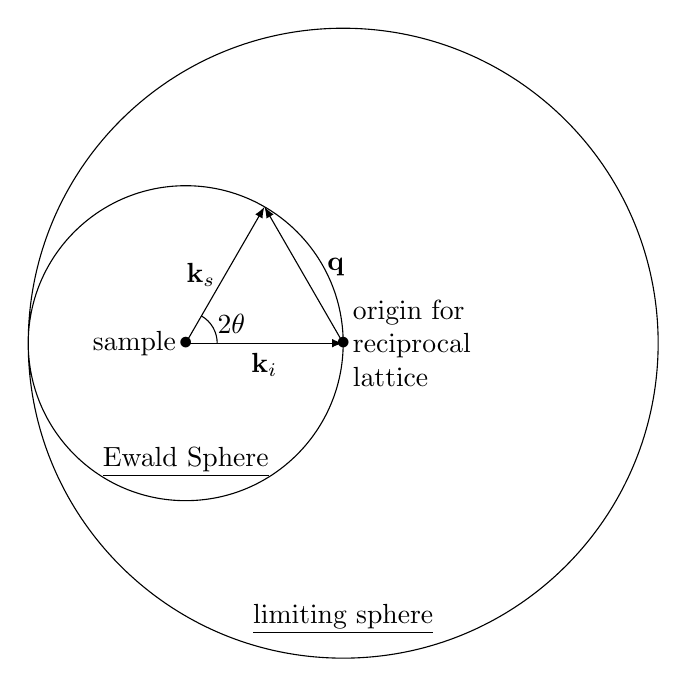
\begin{tikzpicture}
    \def\r {2};
    \draw (0,0) coordinate(O) node{$\bullet$} node[below,left]{sample} circle (\r) ++ (\r,0) coordinate(O2) circle(2*\r);
    \draw[->,>=latex] (0,0) -- ++ (\r,0) node[midway,below] {$\mathbf{k}_i$} node{$\bullet$} node[right,align=left]{origin for\\reciprocal\\lattice};
    \draw[->,>=latex] (0,0) -- ++ (\r*0.5,\r*.866) node[midway,left] {$\mathbf{k}_s$} coordinate(s);
    \draw[->,>=latex] (\r,0) -- (s) node[midway,right,xshift=5,yshift=3] {$\mathbf{q}$};
    \draw (0,-1*\r) node[anchor=south,yshift=5] {\underline{Ewald Sphere}} (\r,-2*\r) node[anchor=south,yshift=5] {\underline{limiting sphere}};
    \draw pic [draw,angle radius=0.4cm] {angle = O2--O--s}; \draw (O) node[anchor=south west,xshift=8]{$2\theta$};
\end{tikzpicture}

\end{document}